\section{Конструкторская часть}

\subsection{Схемы алгоритмов}
На рисунке \ref{fig:base} представлена схема классического умножения матриц.

\newpage
\begin{figure}
\center{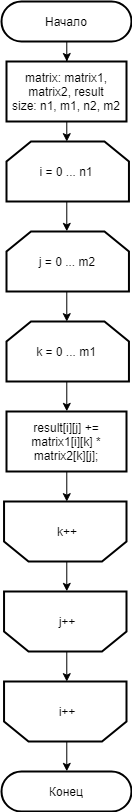
\includegraphics[height=155mm]{pictures/base.png}}
\caption{Схема классического алгоритма умножения матриц}
\label{fig:base}
\end{figure}

На рисунках \ref{fig:vin1}, \ref{fig:vin2}, \ref{fig:vin3}, \ref{fig:vin4} представлена схема алгоритма умножения матриц Винограда.

\begin{figure}
\center{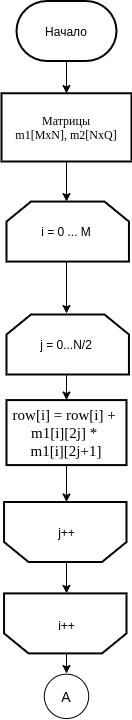
\includegraphics[scale=0.8]{pictures/vin1.png}}
\caption{Схема алгоритма Винограда (часть 1)}
\label{fig:vin1}
\end{figure}

\begin{figure}
\center{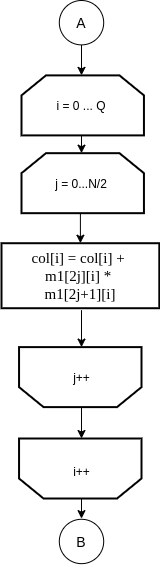
\includegraphics[scale=1]{pictures/vin2.png}}
\caption{Схема алгоритма Винограда (часть 2)}
\label{fig:vin2}
\end{figure}

\begin{figure}
\center{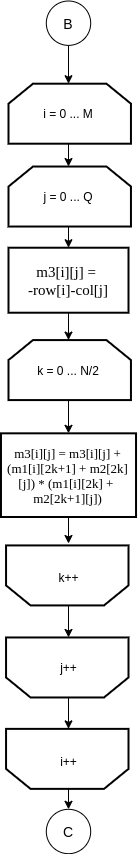
\includegraphics[scale=0.8]{pictures/vin3.png}}
\caption{Схема алгоритма Винограда (часть 3)}
\label{fig:vin3}
\end{figure}

\begin{figure}
\center{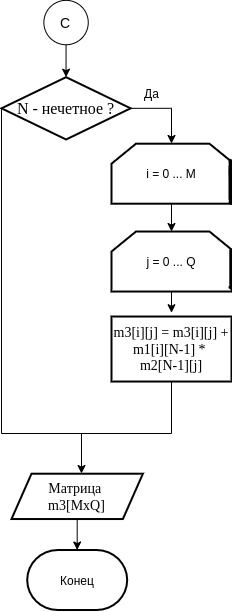
\includegraphics[scale=0.8]{pictures/Inkedvin4_LI.jpg}}
\caption{Схема алгоритма Винограда (часть 4)}
\label{fig:vin4}
\end{figure}

\newpage
На рисунках \ref{fig:vinOpt1}, \ref{fig:vinOpt2}, \ref{fig:vinOpt3}, \ref{fig:vinOpt4} представлена схема оптимизированного алгоритма умножения матриц Винограда.

\begin{figure}
\center{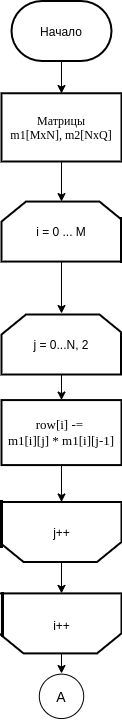
\includegraphics[scale=0.8]{pictures/vinopt1.png}}
\caption{Схема оптимизированного алгоритма Винограда(часть 1)}
\label{fig:vinOpt1}
\end{figure}

\begin{figure}
\center{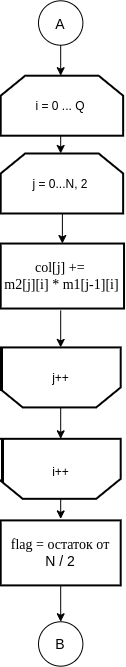
\includegraphics[scale=1]{pictures/vinopt2.png}}
\caption{Схема оптимизированного алгоритма Винограда(часть 2)}
\label{fig:vinOpt2}
\end{figure}

\begin{figure}
\center{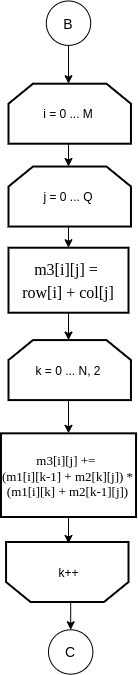
\includegraphics[scale=0.95]{pictures/vinopt3.png}}
\caption{Схема оптимизированного алгоритма Винограда(часть 3)}
\label{fig:vinOpt3}
\end{figure}

\begin{figure}
\center{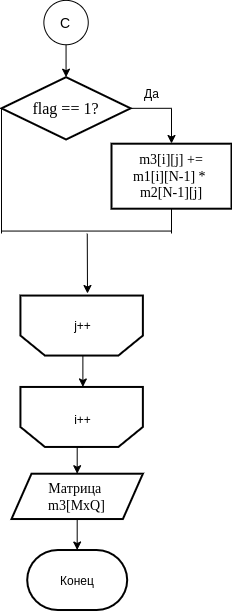
\includegraphics[scale=0.9]{pictures/vinopt4.png}}
\caption{Схема оптимизированного алгоритма Винограда(часть 4)}
\label{fig:vinOpt4}
\end{figure}